\section{Orga}\label{orga}

\begin{frame}[fragile]{R-Befehl zur logistischen Regression}

Die Funktion \texttt{glm} führt die logistische Regression durch.

\begin{Shaded}
\begin{Highlighting}[]
\NormalTok{glm1 <-}\StringTok{ }\KeywordTok{glm}\NormalTok{(Aktienkauf ~}\StringTok{ }\NormalTok{Risikobereitschaft, }
            \DataTypeTok{family =} \KeywordTok{binomial}\NormalTok{(}\StringTok{"logit"}\NormalTok{),}
            \DataTypeTok{data =} \NormalTok{Aktien)}
\end{Highlighting}
\end{Shaded}

\end{frame}

\section{Kap sdjlfk}\label{kap-sdjlfk}

\begin{frame}{Themen pro Termin (insgesamt 44UE Lehre)}

\begin{longtable}[]{@{}rl@{}}
\toprule
Termin & Thema / Kapitel\tabularnewline
\midrule
\endhead
1 & Organisatorisches\tabularnewline
1 & Einführung\tabularnewline
1 & Rahmen\tabularnewline
1 & Daten einlesen\tabularnewline
2 & Datenjudo\tabularnewline
3 & Daten visualisieren\tabularnewline
4 & Fallstudie (z.B. zu `movies')\tabularnewline
5 & Daten modellieren\tabularnewline
5 & Der p-Wert\tabularnewline
6 & Lineare Regression - metrisch\tabularnewline
7 & Lineare Regression - kategorial\tabularnewline
8 & Fallstudie (z.B. zu `titanic' und `affairs')\tabularnewline
9 & Vertiefung 1: Textmining oder Clusteranalyse\tabularnewline
10 & Vertiefung 2: Dimensionsreduktion\tabularnewline
11 & Wiederholung\tabularnewline
\bottomrule
\end{longtable}

\end{frame}

\begin{frame}{Prüfung - Allgemeine Hinweise}

\begin{itemize}
\tightlist
\item
  Die Prüfung besteht aus zwei Teilen

  \begin{itemize}
  \tightlist
  \item
    einer Klausur (50\% der Teilnote)
  \item
    einer Datenanalyse (50\% der Teilnote).
  \end{itemize}
\end{itemize}

\emph{Prüfungsrelevant} ist der gesamte Stoff aus dem Skript und dem
Unterricht mit
\href{https://sebastiansauer.github.io/Praxis_der_Datenanalyse/organisatorisches.html\#prufung}{einigen
Ausnahmen}

Alle Hinweise zur Prüfung gelten nur insoweit nicht anders vom Dozenten
festgelegt.

\end{frame}

\begin{frame}{Lernziele}

\begin{itemize}
\tightlist
\item
  Einen Überblick über die fünf wesentliche Schritte der Datenanalyse
  gewinnen.
\item
  R und RStudio installieren können.
\item
  Einige häufige technische Probleme zu lösen wissen.
\item
  R-Pakete installieren können.
\item
  Einige grundlegende R-Funktionalitäten verstehen.
\item
  Auf die Frage ``Was ist Statistik?'' eine Antwort geben können.
\end{itemize}

\end{frame}

\begin{frame}[fragile]{Datensätze}

Alle Datensätze liegen im Ordner \texttt{data/}, den Sie vom
\href{https://github.com/sebastiansauer/Praxis_der_Datenanalyse}{Github-Repositorium}
herunterladen können.

\end{frame}

\begin{frame}{R und RStudio installieren}


\includegraphics[width=0.10000\textwidth]{../images/Rahmen/Rlogo.png}

\includegraphics[width=0.10000\textwidth]{../images/Rahmen/rstudiologo.png}

\begin{figure}

{\centering 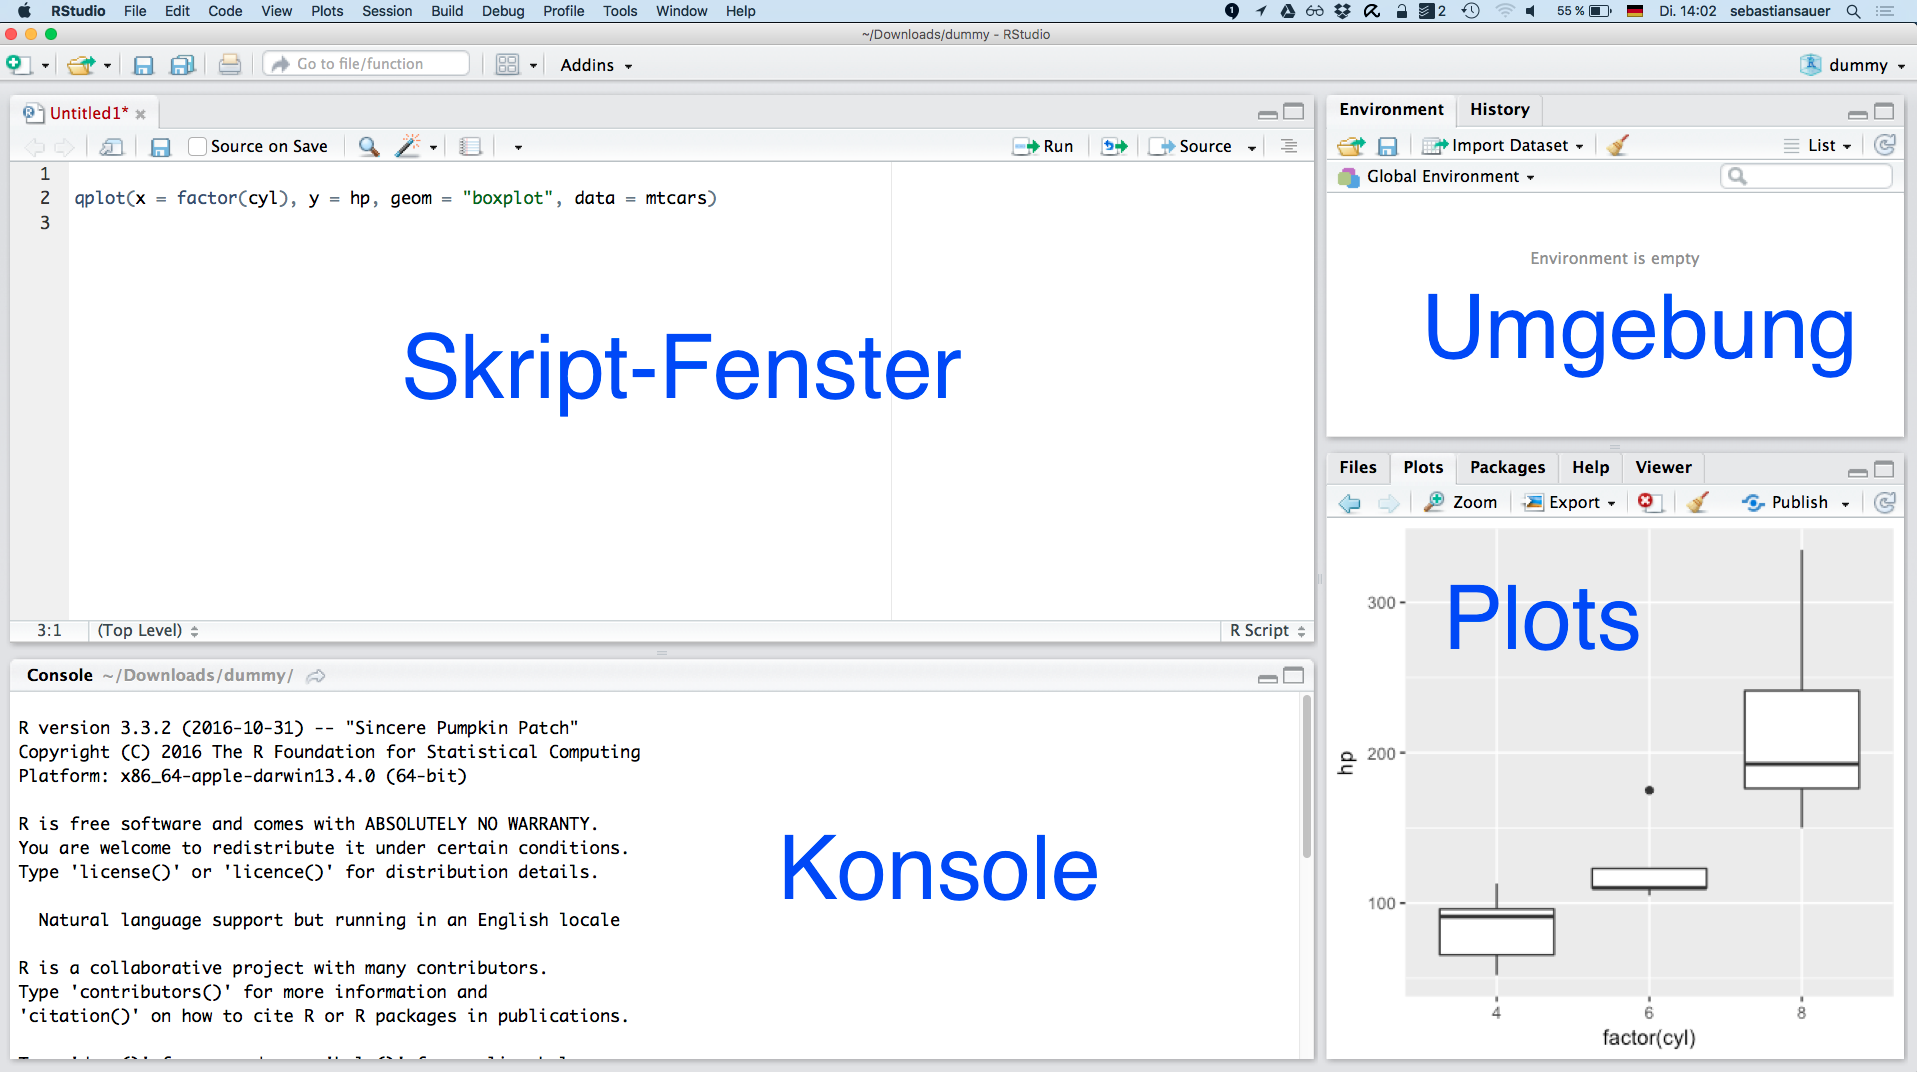
\includegraphics[width=0.5\linewidth]{../images/Rahmen/RStudio-Screenshot} 

}

\caption{RStudio}\label{fig:unnamed-chunk-2}
\end{figure}

\end{frame}

\begin{frame}{Zeilen zählen mit \texttt{n} und \texttt{count}}

\begin{figure}

{\centering 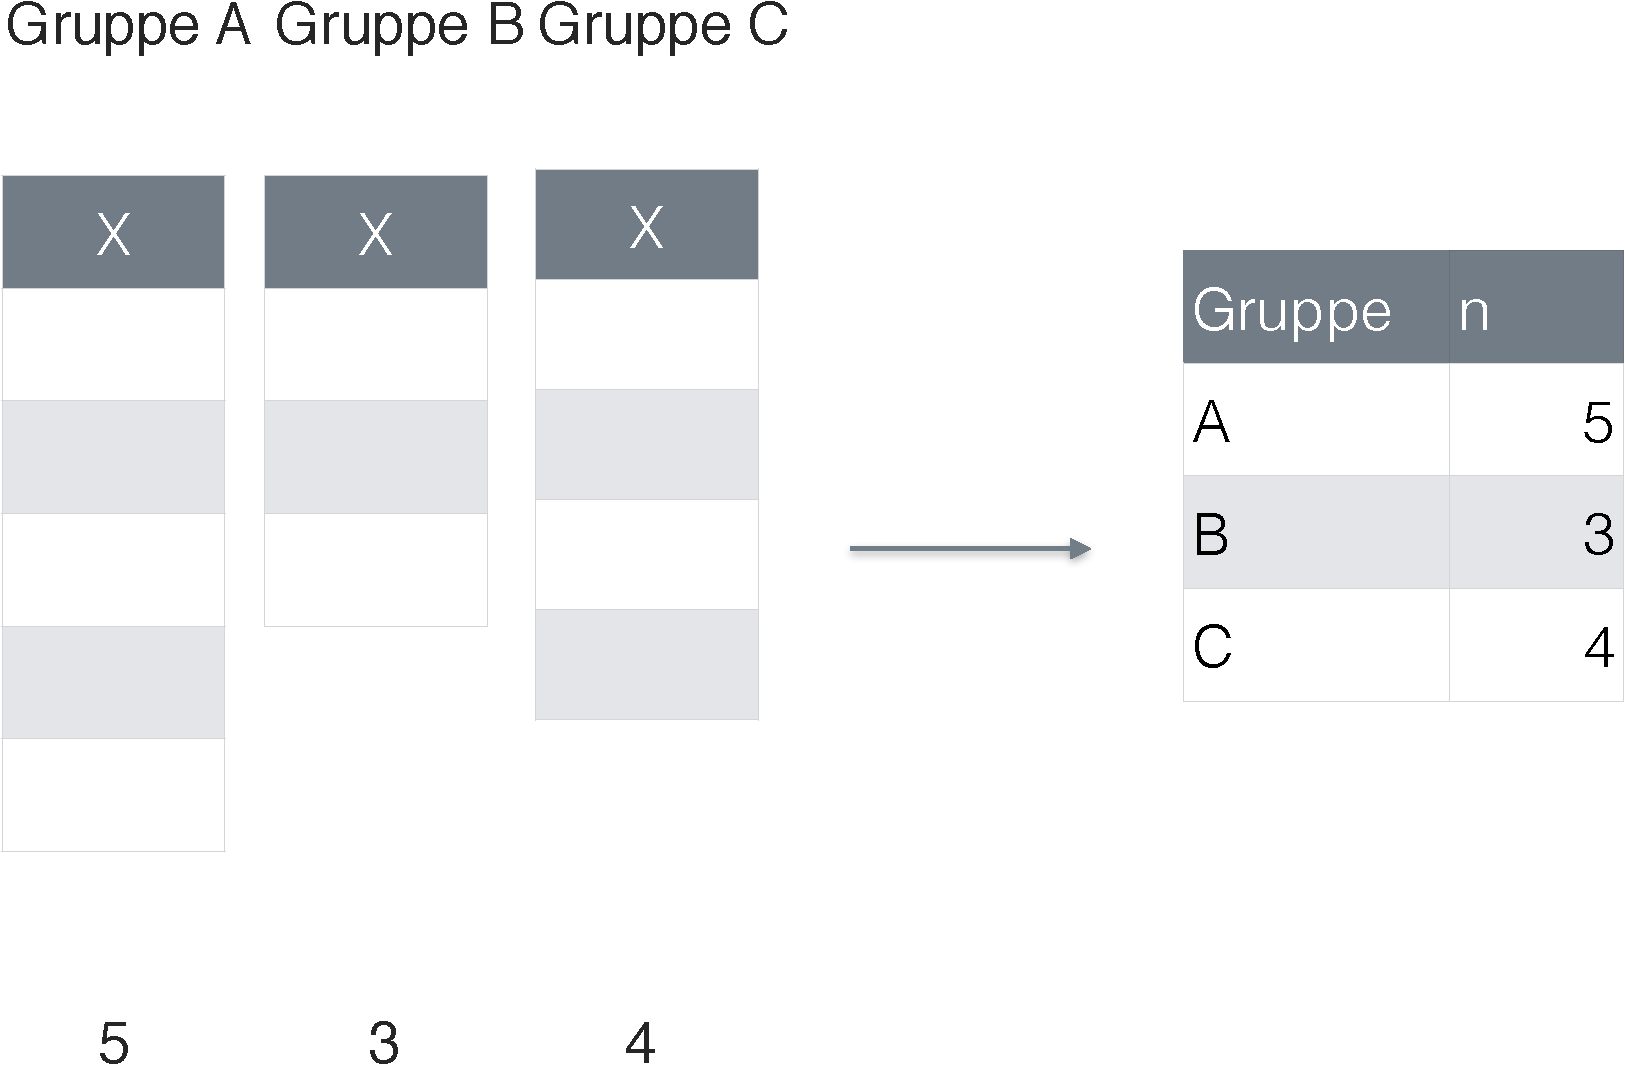
\includegraphics[width=0.8\linewidth]{../images/Datenjudo/count-crop} 

}

\caption{Sinnbild für 'count'}\label{fig:fig-count}
\end{figure}

\end{frame}
